\chapter{Datasets}
\label{chap:dataset}
Accurate and generalizable animal re-identification (Re-ID) system depends on the quality and diversity of datasets used for development and evaluation. This thesis evaluates the proposed approach on publicly available datasets, mostly from WildlifeReID-10k dataset collection\cite{adam2025wildlifereid10kwildlifereidentificationdataset}

\section{WildlifeReID-10k}
WildlifeReID-10k\cite{adam2025wildlifereid10kwildlifereidentificationdataset} is a benchmark dataset collection explicitly curated for evaluating animal Re-ID methods across a variety of species. The primary goal of this dataset is to enable systematic benchmarking of general-purpose animal Re-ID methods. It aggregates \num{37} existing datasets into a unified format to enable easy evaluation. In total, WildlifeReID contains \num{140488} images of \num{10772} unique individuals spanning \num{33} species. The methods described in this thesis were tested on \num{7} datasets from that collection: ATRW (tigers), CowDataset (cows), ElPephants (elephants), CTai (chimps), Chicks4FreeID (chickens), SealID (seals) and SeaStarReID2023 (sea stars). They were chosen because they provide the range of challenges of re-identification and the testing on all \num{37} datasets would be too computationally expensive.  

\begin{figure}[H]
    \centering
    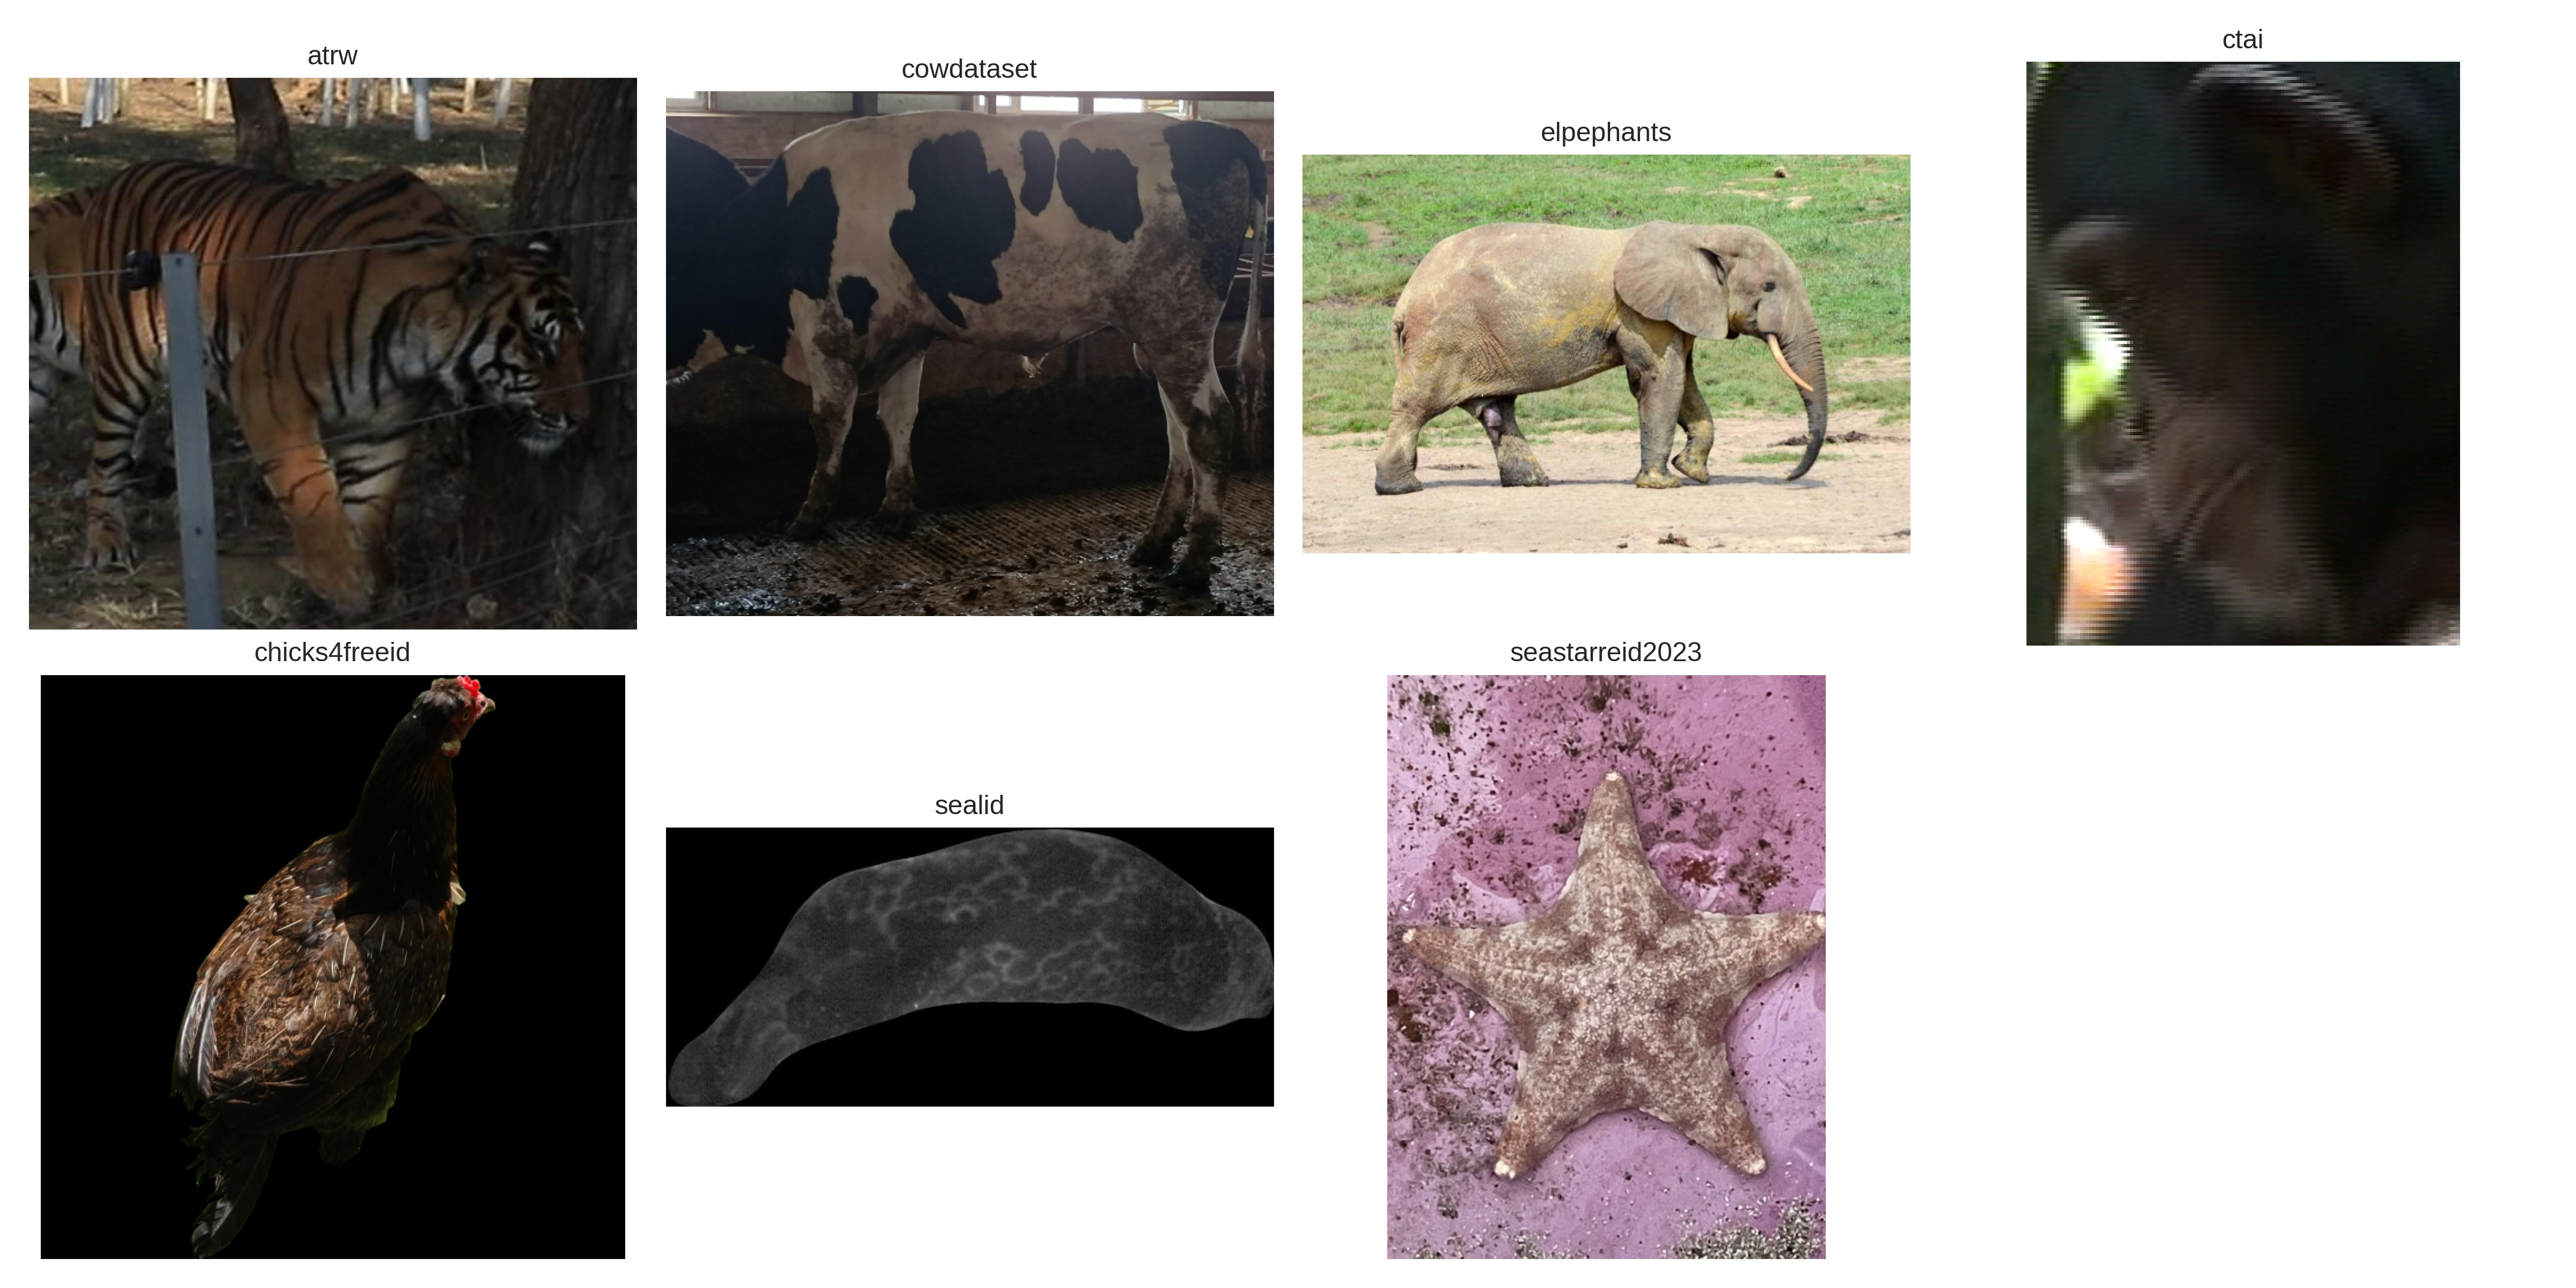
\includegraphics[width=0.95\linewidth]{Figures/dataset_examples_grid.JPG}
    \caption{Example images from the datasets used in this thesis.}
    \label{fig:dataset_examples_grid}
\end{figure}

\subsection{Train/Test Leakage Issues and Split Protocols}
A central (and often not addressed) issue in animal Re-ID evaluation is train-to-test leakage caused by visually almost identical images (for example, consecutive video frames or images from camera traps taken in very quick succession during a single observation) ending up in both train and test sets. There are also mistakes in the datasets, so in some cases there are literal duplicates present. Because of this random splits often result in overly optimistic results that do not reflect real-world generalization.\cite{adam2025wildlifereid10kwildlifereidentificationdataset}

To address this, WildlifeReID-10k proposes two split strategies\cite{adam2025wildlifereid10kwildlifereidentificationdataset}:

\begin{itemize}
    \item \textbf{Time-aware splits}: some of the datasets come with timestamps and this is used to split the images chronologically per identity using a cut-off date so that images from the same encounter do not leak across splits
    \item \textbf{Similarity-aware splits}: when timestamps are not available, an embedding model DINOv2\cite{oquab2024dinov2learningrobustvisual} is used to cluster the images, leveraging the fact that near duplicates should lie close in the embedding space
\end{itemize}

\subsection{MegaDescriptor Training Leakage}
In this thesis I used the MegaDescriptor-L-384 (MD) model for extracting of global embeddings from images, this model was trained on a subset of datasets from WildlifeReID-10k so for those datasets in evaluation I disregarded the time-aware/similarity-aware splits and used the exact same splits that the model was trained on to avoid additional data leaks. Those datasets are: ATRW, CTai and SealID and in later parts of the thesis will be marked with \textbf{*} to signify this. The Exception to this is the ELPephants\cite{Korschens_2019_ICCV} dataset which uses a random split.

\subsection{Datasets Overview}
\begin{table}[H]
\centering
\begin{tabular}{l r r r l}
\hline
\textbf{Dataset} & \textbf{\# images} & \textbf{\# individuals} & \textbf{ratio} & \textbf{split type}\\
\hline
ATRW* & 5,415 & 182 & 29.8 & Original MD split \\
CTai* & 4,662 & 71 & 65.7 & Original MD split \\
SealID* & 2,080 & 57 & 36.5 & Original MD split \\
CowDataset & 1,485 & 13 & 114.2 & Time-aware split \\
Chicks4FreeID & 1,146 & 50 & 22.9 & Similarity-aware split \\
SeaStarReID2023 & 2,187 & 95 & 23.0 & Time-aware split \\
ELPephants & 2078 & 276 & 7.5 & Random split \\
\hline
\end{tabular}
\caption{Datasets used for evaluation in this thesis.}
\label{tab:datasets_used}
\end{table}

\subsection{Class balance visualizations}
Another issue with Re-ID datasets is that they are typically highly imbalanced.

\begin{figure}[H]
    \centering
    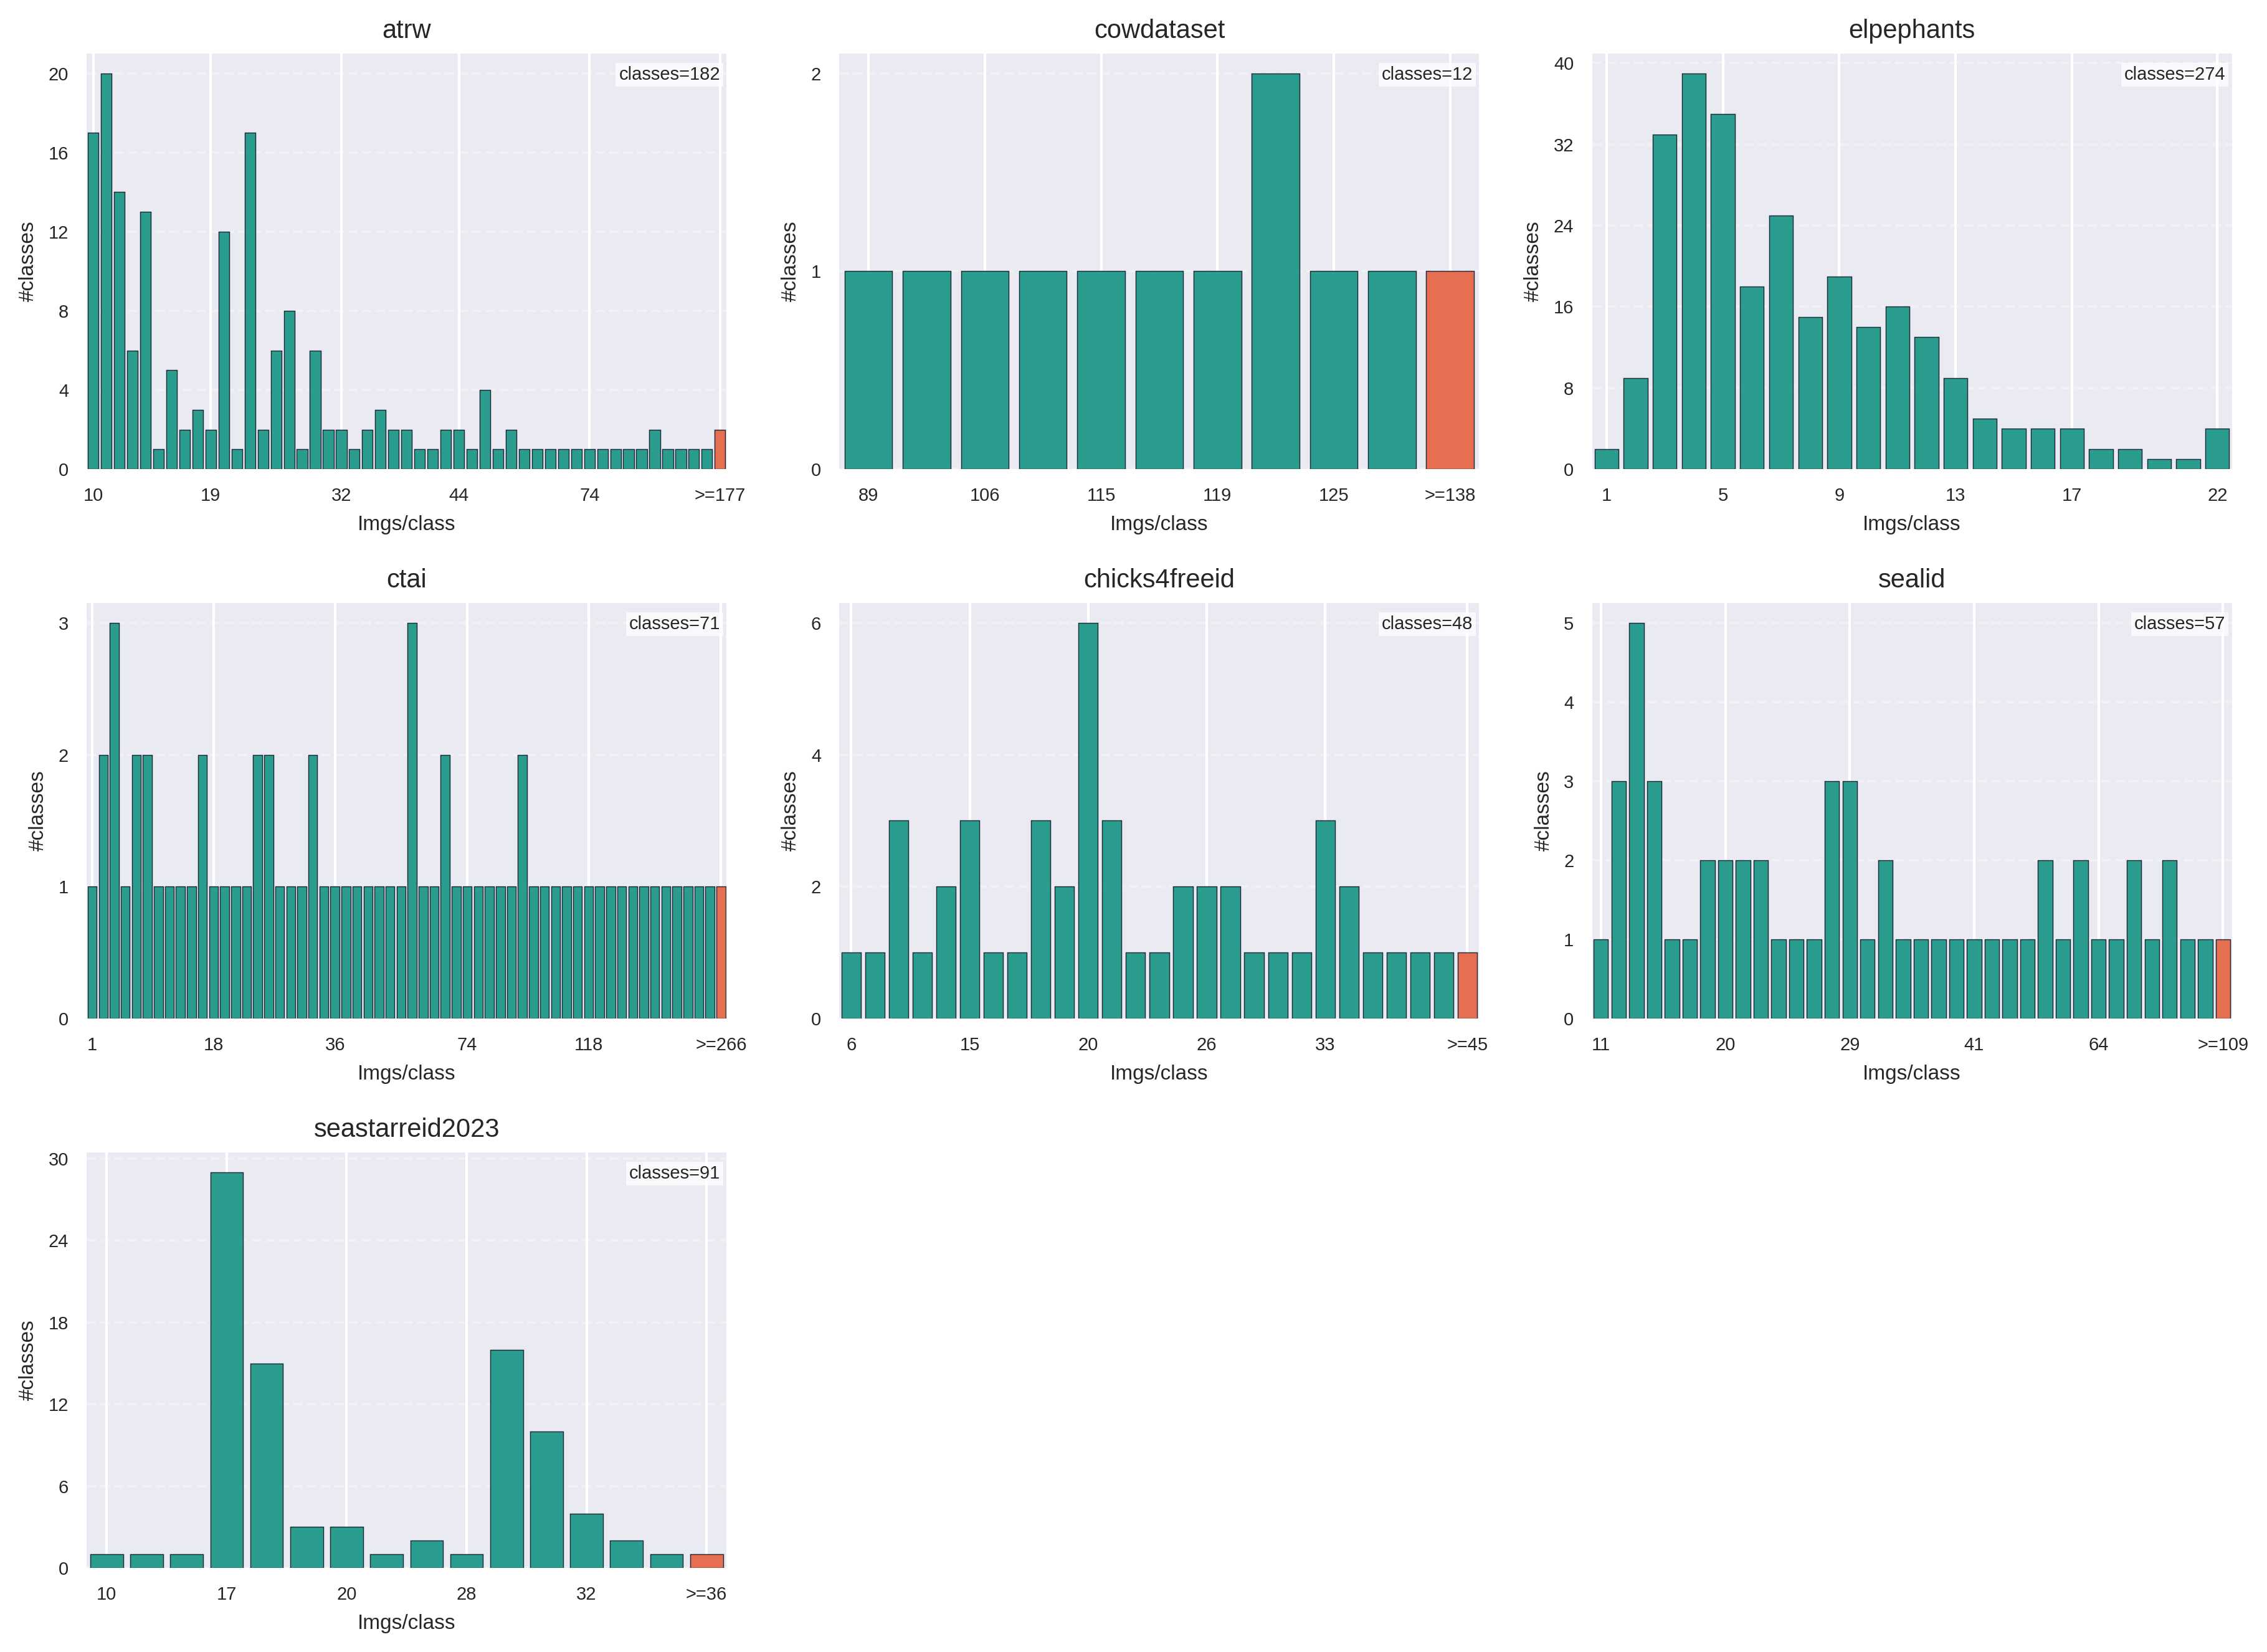
\includegraphics[width=0.95\linewidth]{Figures/class_balance_compact_grid.png}
    \caption{Class balance (number of images per individual) for the datasets used.}
    \label{fig:class_balance_compact_grid}
\end{figure}

